\documentclass[11pt]{article}
\usepackage[margin=1in]{geometry}
\usepackage{amsmath,amssymb}
\usepackage{booktabs}
\usepackage{xcolor}
\usepackage{listings}
\usepackage{tikz}
\usetikzlibrary{positioning,arrows.meta}
\usepackage[hidelinks]{hyperref}

\lstset{basicstyle=\ttfamily\small,columns=fullflexible,keepspaces=true,
        frame=single,rulecolor=\color{gray!50},backgroundcolor=\color{gray!6},
        breaklines=true,showstringspaces=false}

\title{Displacement-Based Frame Sampling\\\large Theory behind \texttt{preprocessing/extract\_frames.py}}
\author{Raphael Pangilinan\\COSC 4346 --- Introduction to Deep Learning}
\date{October 12, 2026}

\begin{document}
\maketitle

\section{Overview}
The corn videos are recorded by a moving GoPro, so consecutive frames are
nearly identical and labeling every frame would be redundant. The script is a
\emph{displacement-based keyframe sampler}: it estimates how far the camera
view moves between consecutive frames, accumulates that movement, and saves a
frame each time the accumulated shift exceeds a threshold, provided the frame
is sharp.

\begin{center}
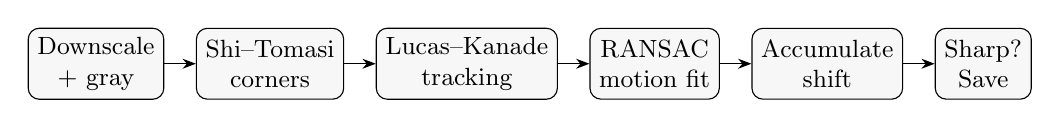
\begin{tikzpicture}[node distance=4mm, every node/.style={draw,rounded corners,
  align=center,font=\small,minimum height=9mm,fill=gray!6}, >=Stealth]
\node (a) {Downscale\\+ gray};
\node[right=of a] (b) {Shi--Tomasi\\corners};
\node[right=of b] (c) {Lucas--Kanade\\tracking};
\node[right=of c] (d) {RANSAC\\motion fit};
\node[right=of d] (e) {Accumulate\\shift};
\node[right=of e] (f) {Sharp?\\Save};
\draw[->] (a)--(b); \draw[->] (b)--(c); \draw[->] (c)--(d);
\draw[->] (d)--(e); \draw[->] (e)--(f);
\end{tikzpicture}
\end{center}

\section{Preprocessing}
Each frame is resized to $640\times360$ and converted to grayscale. Motion
estimation only needs brightness structure, not color, and the reduced frame
has roughly $9\times$ fewer pixels than 1080p. Because the motion measured at
the small scale is proportional to motion at full scale, the threshold keeps
its meaning as a fraction of the frame width. The saved image is the original
full-resolution color frame.

\section{Feature Detection: Shi--Tomasi Corners}
Not every pixel can be tracked. In a flat region, any displacement looks the
same; on an edge, motion is observable only perpendicular to the edge (the
\emph{aperture problem}); at a corner, the patch changes under any
displacement, so its new position is unambiguous.

For each window, the \emph{structure tensor} is built from the image gradients
$I_x, I_y$:
\begin{equation}
M = \sum_{\text{window}} \begin{bmatrix} I_x^2 & I_x I_y \\ I_x I_y & I_y^2 \end{bmatrix}.
\end{equation}
Its eigenvalues $\lambda_1,\lambda_2$ measure how strongly intensity changes in
the two principal directions. Shi and Tomasi~\cite{shi1994} score a window by
$\min(\lambda_1,\lambda_2)$; a corner has both eigenvalues large.
The call \texttt{goodFeaturesToTrack(gray, 300, 0.01, 8)} keeps at most 300
corners, each scoring at least 1\% of the strongest, spaced at least 8 pixels
apart.

\section{Tracking: Pyramidal Lucas--Kanade Optical Flow}
Lucas--Kanade~\cite{lucas1981} assumes \emph{brightness constancy}: a point
keeps its intensity as it moves,
$I(x,y,t) = I(x+u,\,y+v,\,t+1)$. A first-order Taylor expansion gives the
optical flow constraint
\begin{equation}
I_x u + I_y v + I_t = 0,
\end{equation}
one equation in two unknowns. Assuming all pixels in a small window share the
same motion yields an overdetermined system, solved by least squares:
\begin{equation}
\begin{bmatrix} u \\ v \end{bmatrix}
= -M^{-1} \sum_{\text{window}} \begin{bmatrix} I_x I_t \\ I_y I_t \end{bmatrix}.
\end{equation}
The matrix being inverted is the same structure tensor $M$ from the previous
section. The solve is stable only when $M$ is well-conditioned, which is
exactly what the Shi--Tomasi criterion selects for; the two methods are
designed to be used together.

The Taylor approximation holds only for motions of one or two pixels. The
pyramidal implementation~\cite{bouguet2000} estimates motion on a coarse,
downsampled image first and refines it level by level, allowing displacements
of tens of pixels. The returned \texttt{status} array marks which points were
tracked successfully.

\section{Robust Motion Fitting: RANSAC}
The tracked point pairs contain outliers: leaves moving in the wind, false
matches, and points leaving the frame. \texttt{estimateAffinePartial2D} fits a
four-degree-of-freedom similarity transform (rotation $\theta$, uniform scale
$s$, translation $t_x,t_y$):
\begin{equation}
\begin{bmatrix} x' \\ y' \end{bmatrix} =
\begin{bmatrix} s\cos\theta & -s\sin\theta \\ s\sin\theta & s\cos\theta \end{bmatrix}
\begin{bmatrix} x \\ y \end{bmatrix} +
\begin{bmatrix} t_x \\ t_y \end{bmatrix}.
\end{equation}
RANSAC~\cite{fischler1981} makes the fit robust:
\begin{enumerate}
  \item Randomly pick the minimal sample (two point pairs) and fit a transform.
  \item Count the \emph{inliers}: pairs that agree with it within a few pixels.
  \item Repeat, keep the transform with the most inliers, and refit it on all of them.
\end{enumerate}
Ordinary least squares would be pulled toward the outliers; RANSAC ignores
them. The per-frame displacement is the magnitude of the translation,
$d = \sqrt{t_x^2 + t_y^2}$, since the camera moves both horizontally and
vertically.

\section{Accumulation and Threshold}
Per-frame displacements are a few pixels. The script sums them since the last
saved frame and saves when the total reaches
$0.5 \times 640 = 320$ pixels. At that point the view has slid about half a
frame, so neighboring saved frames overlap by about half or less. Sampling therefore depends on \emph{distance covered} rather than
\emph{elapsed time}: slow and fast walking produce similarly spaced frames,
which is the main advantage over sampling one frame per second.

Two limitations apply. Small per-frame errors accumulate (\emph{drift}), but
this is harmless because the sum resets at every saved frame. And a single
translation ignores \emph{parallax}: near plants move across the image faster
than far ones, so RANSAC follows whichever depth layer has the most points.
That is sufficient for deciding when to sample, but it is not a metric
measurement of how far the camera traveled.

\section{Blur Rejection: Variance of the Laplacian}
The Laplacian $\nabla^2 I = \partial^2 I/\partial x^2 + \partial^2 I/\partial y^2$
responds strongly at sharp edges. A sharp image has many strong responses of
both signs and therefore a high response variance; motion blur spreads edges
out and lowers it~\cite{pech2000}. When a frame is due to be saved but scores
below \texttt{MIN\_SHARP} $=50$, the script waits for the next sharp frame.
The score depends on scene content, so the threshold must be tuned per
dataset.

\section{Parameters and Results}
\begin{center}
\begin{tabular}{lll}
\toprule
Parameter & Value & Meaning \\
\midrule
\texttt{SMALL\_W}, \texttt{SMALL\_H} & $640\times360$ & resolution for motion estimation \\
\texttt{MOVE\_FRAC} & 0.5 & save after shifting this fraction of the width \\
\texttt{MIN\_SHARP} & 50 & minimum Laplacian variance \\
\bottomrule
\end{tabular}
\end{center}

Run on all 40 videos (24\,fps), the script kept 463 of 16{,}293 frames
(about 3\%): 237 from the 2-foot camera and 226 from the 4-foot camera, or 9
to 15 frames per video.

\section{Core Code}
\begin{lstlisting}[language=Python]
def shift_between(prev_gray, gray):
    pts_old = cv2.goodFeaturesToTrack(prev_gray, 300, 0.01, 8)
    if pts_old is None:
        return 0.0
    pts_new, status, _ = cv2.calcOpticalFlowPyrLK(prev_gray, gray, pts_old, None)
    found = status.ravel() == 1
    if found.sum() < 10:
        return 0.0
    M, _ = cv2.estimateAffinePartial2D(pts_old[found], pts_new[found],
                                       method=cv2.RANSAC)
    return 0.0 if M is None else float(np.hypot(M[0, 2], M[1, 2]))
\end{lstlisting}

\section*{Further Reading}
\begin{itemize}\raggedright
  \item R.~Szeliski, \emph{Computer Vision: Algorithms and Applications}, 2nd ed.,
        free at \url{https://szeliski.org/Book}. Feature detection (Ch.~7),
        motion estimation and optical flow (Chs.~8--9).
  \item OpenCV tutorials, \emph{Shi-Tomasi Corner Detector \& Good Features to Track}
        and \emph{Optical Flow}, \url{https://docs.opencv.org}.
  \item A.~Rosebrock, ``Blur detection with OpenCV,'' PyImageSearch, 2015.
\end{itemize}

\begin{thebibliography}{9}
\bibitem{shi1994} J.~Shi and C.~Tomasi, ``Good features to track,'' in
  \emph{Proc.\ IEEE CVPR}, 1994, pp.~593--600.
\bibitem{lucas1981} B.~D.~Lucas and T.~Kanade, ``An iterative image
  registration technique with an application to stereo vision,'' in
  \emph{Proc.\ IJCAI}, 1981, pp.~674--679.
\bibitem{bouguet2000} J.-Y.~Bouguet, ``Pyramidal implementation of the Lucas
  Kanade feature tracker,'' Intel Corporation, Microprocessor Research Labs,
  Tech.\ Rep., 2000.
\bibitem{fischler1981} M.~A.~Fischler and R.~C.~Bolles, ``Random sample
  consensus: A paradigm for model fitting with applications to image analysis
  and automated cartography,'' \emph{Communications of the ACM}, vol.~24,
  no.~6, pp.~381--395, 1981.
\bibitem{pech2000} J.~L.~Pech-Pacheco, G.~Crist\'obal, J.~Chamorro-Mart\'inez,
  and J.~Fern\'andez-Valdivia, ``Diatom autofocusing in brightfield
  microscopy: A comparative study,'' in \emph{Proc.\ ICPR}, 2000,
  pp.~314--317.
\end{thebibliography}

\end{document}
